
% 2018 KTS
% Dancing links package

\documentclass[xcolor=svgnames]{beamer}

\usetheme[titleformat=smallcaps,subsectionpage=progressbar]{metropolis}
\metroset{outer/progressbar=head}

\usepackage{fancyvrb}
\hypersetup{pdfencoding=auto}

\usepackage{sudoku-dlx}
\usepackage{pentominoes}
\usepackage{queens}


% title
\title{Dancing links package}
\subtitle{Exact cover solver using Lua\TeX }
\date{February 3, 2018}
\author{Soojin Nam}
\institute{The Korean \TeX\ Society}
\titlegraphic{\hfill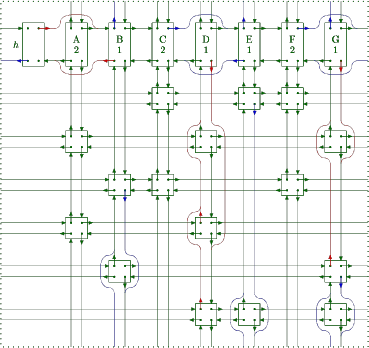
\includegraphics[height=3.2cm]{imgs/cdance-4.png}}


%%
\begin{document}

\maketitle

%
\begin{frame}{Table of contents}
  \setbeamertemplate{section in toc}[sections numbered]
  \tableofcontents
\end{frame}


%%
\section{Exact cover problem}

\let\a\alert
%
\begin{frame}{Exact cover problem}
\Large\boldmath
$$
\bordermatrix{
  \strut&&&&&&&\cr
  &0&0&1&0&1&0&0\cr
  &1&0&0&1&0&0&1\cr
  &0&1&1&0&0&1&0\cr
  &1&0&0&1&0&1&0\cr
  &0&1&0&0&0&0&1\cr
  &0&0&0&1&1&0&1}
$$
\end{frame}

%
\begin{frame}{Exact cover problem}
\Large\boldmath
$$
\bordermatrix{
  &2&2&2&3&2&2&3\cr
  &0&0&1&0&1&0&0\cr
  &1&0&0&1&0&0&1\cr
  &0&1&1&0&0&1&0\cr
  &1&0&0&1&0&1&0\cr
  &0&1&0&0&0&0&1\cr
  &0&0&0&1&1&0&1}
$$
\end{frame}

%
\begin{frame}{Exact cover problem}
\Large\boldmath
$$
\bordermatrix{
  &1&1&1&1&1&1&1\cr
  &0&0&1&0&1&0&0\cr
  &1&0&0&1&0&0&1\cr
  &0&1&1&0&0&1&0\cr
  &1&0&0&1&0&1&0\cr
  &0&1&0&0&0&0&1\cr
  &0&0&0&1&1&0&1}
$$
\end{frame}

%
\begin{frame}{Exact cover problem}
\Large\boldmath
$$
\bordermatrix{
  &1&1&1&1&1&1&1\cr
  &\a0&\a0&\a1&\a0&\a1&\a0&\a0\cr
  &1&0&0&1&0&0&1\cr
  &0&1&1&0&0&1&0\cr
  &\a1&\a0&\a0&\a1&\a0&\a1&\a0\cr
  &\a0&\a1&\a0&\a0&\a0&\a0&\a1\cr
  &0&0&0&1&1&0&1}
$$
\end{frame}

%
\begin{frame}{Exact cover problem}
\Large\boldmath
  \begin{figure}[!htb]
    \hskip-17mm\begin{minipage}{.7\textwidth}
      \centering
      $\bordermatrix{
  \strut&&&&&&&\cr
  &0&0&1&0&1&0&0\cr
  &1&0&0&1&0&0&1\cr
  &0&1&1&0&0&1&0\cr
  &1&0&0&1&0&1&0\cr
  &0&1&0&0&0&0&1\cr
  &0&0&0&1&1&0&1}\ \Rightarrow$
    \end{minipage}%
    \begin{minipage}{.3\textwidth}
      \centering
  $
  \begin{array}{ccccccc}
    A & B & C & D & E & F & G\\
    \hline
    C & E &&&&&\\
    A & D & G &&&&\\
    B & C & F &&&&\\
    A & D & F &&&&\\
    B & G &&&&&\\
    D & E & G &&&&
  \end{array}
  $
    \end{minipage}
\end{figure}
\end{frame}

\renewcommand\arraystretch{1.3}
%
\begin{frame}{Algorithm X}
\Large\boldmath
  $$
  \begin{array}{ccccccc}
    A & B & C & D & E & F & G\\
    \hline
    C & E &&&&&\\
    A & D & G &&&&\\
    B & C & F &&&&\\
    A & D & F &&&&\\
    B & G &&&&&\\
    D & E & G &&&&
  \end{array}
  $$
\end{frame}

%
\begin{frame}{Algorithm X}
\Large\boldmath
  $$
  \begin{array}{ccccccc}
    \a A & B & C & \a D & E & F & \a G\\
    \hline
    C & E &&&&&\\
    \a A & \a D & \a G &&&&\\
    B & C & F &&&&\\
    A & D & F &&&&\\
    B & G &&&&&\\
    D & E & G &&&&
  \end{array}
  $$
\end{frame}

\def\lg{\color{LightGray}}
%
\begin{frame}{Algorithm X}
\Large\boldmath
  $$
  \begin{array}{ccccccc}
    \a A & B & C & \a D & E & F & \a G\\
    \hline
    C & E &&&&&\\
    \a A & \a D & \a G &&&&\\
    B & C & F &&&&\\
    \lg A & \lg D & \lg F &&&&\\
    \lg B & \lg G &&&&&\\
    \lg D & \lg E & \lg G &&&&
  \end{array}
  $$
\end{frame}

%
\begin{frame}{Algorithm X}
\Large\boldmath
  $$
  \begin{array}{ccccccc}
    \a A & B & \a C & \a D & \a E & F & \a G\\
    \hline
    \a C & \a E &&&&&\\
    \a A & \a D & \a G &&&&\\
    B & C & F &&&&\\
    \lg A & \lg D & \lg F &&&&\\
    \lg B & \lg G &&&&&\\
    \lg D & \lg E & \lg G &&&&
  \end{array}
  $$
\end{frame}

%
\begin{frame}{Algorithm X}
  \Large\boldmath
  $$
  \begin{array}{ccccccc}
    \a A & B & \a C & \a D & \a E & F & \a G\\
    \hline
    \a C & \a E &&&&&\\
    \a A & \a D & \a G &&&&\\
    \lg B & \lg C & \lg F &&&&\\
    \lg A & \lg D & \lg F &&&&\\
    \lg B & \lg G &&&&&\\
    \lg D & \lg E & \lg G &&&&
  \end{array}
  $$
\end{frame}

%
\begin{frame}{Algorithm X}
\Large\boldmath
  $$
  \begin{array}{ccccccc}
    A & B & C & D & E & F & G\\
    \hline
    C & E &&&&&\\
    A & D & G &&&&\\
    B & C & F &&&&\\
    A & D & F &&&&\\
    B & G &&&&&\\
    D & E & G &&&&
  \end{array}
  $$
\end{frame}

%
\begin{frame}{Algorithm X}
\Large\boldmath
  $$
  \begin{array}{ccccccc}
    \a A & B & C & \a D & E & \a F & G\\
    \hline
    C & E &&&&&\\
    A & D & G &&&&\\
    B & C & F &&&&\\
    \a A & \a D & \a F &&&&\\
    B & G &&&&&\\
    D & E & G &&&&
  \end{array}
  $$
\end{frame}

%
\begin{frame}{Algorithm X}
\Large\boldmath
  $$
  \begin{array}{ccccccc}
    \a A & B & C & \a D & E & \a F & G\\
    \hline
    C & E &&&&&\\
    \lg A & \lg D & \lg G &&&&\\
    \lg B & \lg C & \lg F &&&&\\
    \a A & \a D & \a F &&&&\\
    B & G &&&&&\\
    \lg D & \lg E & \lg G &&&&
  \end{array}
  $$
\end{frame}

%
\begin{frame}{Algorithm X}
\Large\boldmath
  $$
  \begin{array}{ccccccc}
    \a A & B & \a C & \a D & \a E & \a F & G\\
    \hline
    \a C & \a E &&&&&\\
    \lg A & \lg D & \lg G &&&&\\
    \lg B & \lg C & \lg F &&&&\\
    \a A & \a D & \a F &&&&\\
    B & G &&&&&\\
    \lg D & \lg E & \lg G &&&&
  \end{array}
  $$
\end{frame}

%
\begin{frame}{Algorithm X}
\Large\boldmath
$$
  \begin{array}{ccccccc}
    \a A & \a B & \a C & \a D & \a E & \a F & \a G\\
    \hline
    \a C & \a E &&&&&\\
    \lg A & \lg D & \lg G &&&&\\
    \lg B & \lg C & \lg F &&&&\\
    \a A & \a D & \a F &&&&\\
    \a B & \a G &&&&&\\
    \lg D & \lg E & \lg G &&&&
  \end{array}
  $$
\end{frame}

%
\begin{frame}{Algorithm X}
\Large\boldmath
  $$
  \begin{array}{ccccccc}
    A & B & C & D & E & F & G\\
    \hline
    C & E &&&&&\\
    A & D & G &&&&\\
    B & C & F &&&&\\
    A & D & F &&&&\\
    B & G &&&&&\\
    D & E & G &&&&
  \end{array}
  $$
\end{frame}


%%
\section{Dancing links}

%
\begin{frame}{Dancing links}
%  \begin{itemize}
%  \item A technique that efficiently implements
%    \textsc{Algorithm X}
%  \item \textsc{Algorithm X} finds all solutions to
%    the exact cover problem.
%  \end{itemize}
  \centering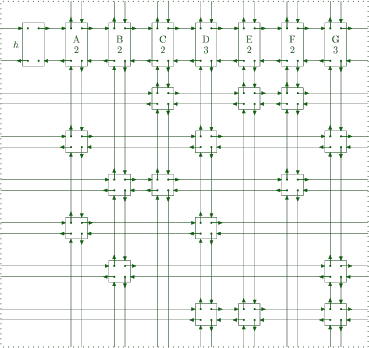
\includegraphics[height=7.5cm]{imgs/cdance-2.png}
\end{frame}

%
\begin{frame}{Dancing links}
%  \begin{itemize}
%  \item A technique that efficiently implements
%    \textsc{Algorithm X}
%  \item \textsc{Algorithm X} finds all solutions to
%    the exact cover problem.
%  \end{itemize}
  \centering\includegraphics[height=7.5cm]{imgs/cdance-3.png}
\end{frame}

%
\begin{frame}{Dancing links}
%  \begin{itemize}
%  \item A technique that efficiently implements
%    \textsc{Algorithm X}
%  \item \textsc{Algorithm X} finds all solutions to
%    the exact cover problem.
%  \end{itemize}
  \centering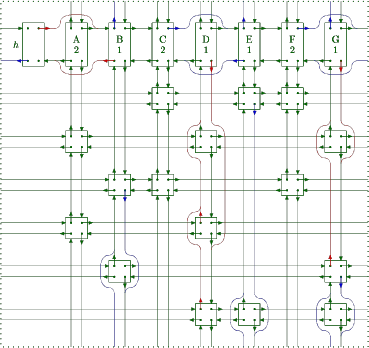
\includegraphics[height=7.5cm]{imgs/cdance-4.png}
\end{frame}

%
\begin{frame}{\texttt{lua-dancing-links}}
\begin{center}
  \href{https://github.com/sjnam/lua-dancing-links}
       {github.com/sjnam/lua-dancing-links}
\end{center}
$$
  \begin{array}{ccccccc}
    A & B & C & D & E & F & G\\
    C & E &&&&&\\
    A & D & G &&&&\\
    B & C & F &&&&\\
    A & D & F &&&&\\
    B & G &&&&&\\
    D & E & G &&&&
  \end{array}
$$
\end{frame}


%%
\section{Pentominoes}

%
\begin{frame}[fragile]{Pentominoes}
  \centering\includegraphics[height=5cm]{imgs/pent.png}
\end{frame}

%
\begin{frame}[fragile]{Pentominoes, 6x10}
\begin{verbatim}
\usepackage{pentominoes}
\pentominoes{1.8em}{6}{10}{1}.
\end{verbatim}  

\pentominoes{2em}{6}{10}{1}.

\end{frame}

%
\begin{frame}{Pentominoes, 8x8}
\pentominoes{1.8em}{8}{8}{1}.
\end{frame}


%%
\section{Sudoku}

%
\begin{frame}[fragile]{Sudoku}
\begin{verbatim}
\sudoku {9.......6.3.4....9...915.8..8.5..7..%
..3.9.4....2..1.9.32176....6..1.2.3.8...5...1}
\end{verbatim}  
\begin{center}
  \sudoku{9.......6.3.4....9...915.8..8.5..7..%
    ..3.9.4....2..1.9.32176....6..1.2.3.8...5...1}
\end{center}
\end{frame}

%
\begin{frame}[fragile]{Sudoku}
\begin{verbatim}
\sudoku*{9.......6.3.4....9...915.8..8.5..7..%
..3.9.4....2..1.9.32176....6..1.2.3.8...5...1}
\end{verbatim}
\begin{center}
  \sudoku*{9.......6.3.4....9...915.8..8.5..7..%
    ..3.9.4....2..1.9.32176....6..1.2.3.8...5...1}
\end{center}
\end{frame}


%%
\section{N-Queens}

%
\begin{frame}[fragile]{n-queens}
\begin{verbatim}
\usepackage{queens}
\queens{8}{2}.
\end{verbatim}
\vspace{-10mm}
\queens{8}{2}.
\end{frame}


%
\begin{frame}{References}
  \begin{itemize}
  \item \href{http://www-cs-faculty.stanford.edu/~knuth/fasc5c.ps.gz}
    {\textsc{The Art of Computer Programming Pre-Fascicle 5c}}
  \item \href{https://github.com/sjnam/lua-dancing-links}
    {github.com/sjnam/lua-dancing-links}
  \end{itemize}
\end{frame}

%
\begin{frame}[standout]
  Questions?
\end{frame}

\end{document}
